\documentclass{article}\usepackage[]{graphicx}\usepackage[]{color}
%% maxwidth is the original width if it is less than linewidth
%% otherwise use linewidth (to make sure the graphics do not exceed the margin)
\makeatletter
\def\maxwidth{ %
  \ifdim\Gin@nat@width>\linewidth
    \linewidth
  \else
    \Gin@nat@width
  \fi
}
\makeatother

\definecolor{fgcolor}{rgb}{0.345, 0.345, 0.345}
\newcommand{\hlnum}[1]{\textcolor[rgb]{0.686,0.059,0.569}{#1}}%
\newcommand{\hlstr}[1]{\textcolor[rgb]{0.192,0.494,0.8}{#1}}%
\newcommand{\hlcom}[1]{\textcolor[rgb]{0.678,0.584,0.686}{\textit{#1}}}%
\newcommand{\hlopt}[1]{\textcolor[rgb]{0,0,0}{#1}}%
\newcommand{\hlstd}[1]{\textcolor[rgb]{0.345,0.345,0.345}{#1}}%
\newcommand{\hlkwa}[1]{\textcolor[rgb]{0.161,0.373,0.58}{\textbf{#1}}}%
\newcommand{\hlkwb}[1]{\textcolor[rgb]{0.69,0.353,0.396}{#1}}%
\newcommand{\hlkwc}[1]{\textcolor[rgb]{0.333,0.667,0.333}{#1}}%
\newcommand{\hlkwd}[1]{\textcolor[rgb]{0.737,0.353,0.396}{\textbf{#1}}}%

\usepackage{framed}
\makeatletter
\newenvironment{kframe}{%
 \def\at@end@of@kframe{}%
 \ifinner\ifhmode%
  \def\at@end@of@kframe{\end{minipage}}%
  \begin{minipage}{\columnwidth}%
 \fi\fi%
 \def\FrameCommand##1{\hskip\@totalleftmargin \hskip-\fboxsep
 \colorbox{shadecolor}{##1}\hskip-\fboxsep
     % There is no \\@totalrightmargin, so:
     \hskip-\linewidth \hskip-\@totalleftmargin \hskip\columnwidth}%
 \MakeFramed {\advance\hsize-\width
   \@totalleftmargin\z@ \linewidth\hsize
   \@setminipage}}%
 {\par\unskip\endMakeFramed%
 \at@end@of@kframe}
\makeatother

\definecolor{shadecolor}{rgb}{.97, .97, .97}
\definecolor{messagecolor}{rgb}{0, 0, 0}
\definecolor{warningcolor}{rgb}{1, 0, 1}
\definecolor{errorcolor}{rgb}{1, 0, 0}
\newenvironment{knitrout}{}{} % an empty environment to be redefined in TeX

\usepackage{alltt}

\usepackage[top=1in, bottom=1in, left=1in, right=1in]{geometry}
\usepackage{float}
\usepackage{graphics}
\usepackage[T1]{fontenc}
\usepackage[english]{babel}
\usepackage{graphicx}
\usepackage{natbib}
\renewcommand{\ni}{\noindent}
\usepackage{enumerate}
\usepackage{url}
\usepackage{ulem}
\usepackage{amstext}
\usepackage{amssymb}

\setlength{\parindent}{0em}


% comment colors causing compilation problems
\usepackage[usenames,dvipsnames]{xcolor}
\newcommand{\hh}[1]{{\color{ForestGreen} #1}}
\newcommand{\km}[1]{{\color{Orange} #1}}

\newcommand{\V}[1]{\text{Var}\left(#1\right)}
\IfFileExists{upquote.sty}{\usepackage{upquote}}{}
\begin{document}
\tableofcontents
\newpage


%load packages that will be invisible on slides



%opening
\title{A \texttt{shiny} New Opportunity for Interaction with Big Data in Undergraduate Education}
%\subtitle{ }
\author{Karsten Maurer \\ Iowa State University, Ames, IA, USA}

\maketitle


% \date{Received: date / Accepted: date}

 \begin{abstract}
As the availability of truly massive data sets proliferates it is enticing to incorporate these data sources into the curriculum of an undergraduate statistics course.  Major barriers exist for interacting with big data due to the computationally intense nature of working with large databases.  Difficulties include gaining access to the database, interacting with database management software and obtaining summary statistics or manageable subsamples from the database for student use.  This paper describes a pair of web based applications, the Shiny Database Sampler and the Shiny Database Aggregator, which allows instructors to bypass these barriers using simple JavaScript based tools constructed using R and the R packages \texttt{shiny} and \texttt{RMySQL}. The Shiny Database Sampler allows instructors and/or students to obtain smaller subsamples from databases, using a variety of random sampling schemes. The Shiny Database Aggregator ...
 \end{abstract}

\section{Introduction}
\begin{itemize}
\item Write Intro Last
\end{itemize}

\hh{Lit Review is part of the intro; general outline of the intro should be something like
\begin{itemize}
\item: Motivation of what do we do?
\item What has been done? - that's where the part of the lit review comes in
\item Why is what we are doing relevant, i.e. where are the holes in the lit review - that can be mixed with the previous item
\item Outline of the structure of the rest of the paper
\end{itemize}}

%-----------------------------------------------------------------------------------
% \section{Literature Review}
% \begin{itemize}
% \item 
% \end{itemize}

%-----------------------------------------------------------------------------------
\section{Shiny Database Sampler}
\begin{itemize}
\item Brief intro the functionality goals for the tool
\end{itemize}

%%%-----------------------------------------------------------------------------------
\subsection{Layout and Functionality}

\underline{sampling options}
\begin{itemize}
\item database: recmiler, accidents, census
\item type: SRS, stratified
\item sample size
\item seed: why seed available
\end{itemize}

\vspace{.1in}

\underline{data summaries}
\begin{itemize}
\item table: sortable, searchable
\item summary statistics: basic, broken down by strata if stratified sample taken
\item plots: specify 1 or 2 variables and variable types to generate default plot types
\end{itemize}

\vspace{.1in}

\underline{Export}
\begin{itemize}
\item to csv file
\end{itemize}

\vspace{.1in}

%%%-----------------------------------------------------------------------------------
\subsection{Applications}

\begin{itemize}
\item Used in introductory statistics course for lab and course project
\item Project Use: students pick question then run mock survey using sampler tool
\item Lab Use: description of lab (perhaps relocate paragraph 2 of next section here)
\end{itemize}

%%%-----------------------------------------------------------------------------------
\subsection{Student Response Survey Following Lab Application}

As discussed above, the Shiny Database Sampler was designed for student use on course assignments. We were interested to learn student opinions about using the tool. Specifically we wanted know if students find the tool easy to operate, if they see the connection to sampling concepts and if they find the data engaging. \km{These topics are selected to assess the quality of the Shiny Database Sampler with respect to the interface design and educational value.}
\hh{slow down - here we will need about one paragraph each for the topics. Start by a more formal definition of what you mean by the topic - give a reference - and how it helps with student learning. }
\km{\textbf{citation on HCI for why ease of use is important}.  The GAISE guidelines recommend that technological tools should be used to help teach statistical concepts and that the use of real data is important for student engagement, hence we focus on these topics \citep{GAISEcollege}. } \\

Student responses were collected in an anonymous survey following a group lab assignment that required students of Stat 104, Introduction to Statistics, at Iowa State University to use the Shiny Database Sampler tool. Six sections of Stat 104 students were surveyed. The students were informed that the survey was not required and that no penalties or rewards were affiliated with its completion.  Of the 320 students attending lab, 265 completed the survey. 

%-------------------------------------------------------------------------
 \subsubsection{Lab Overview} 

The lab that utilized the Shiny Database Sampler was designed for students to think critically about sampling approaches, then use the tool allowed to treat the large database as 
a population from which to obtain survey data. Students were asked to consider the following pair of hypothetical situations:

\begin{enumerate}
\item Suppose that our goal is to estimate the mean age of all US residents. Similar to polling organizations we have a budget that allows us to survey around 1000 people. To collect our sample we decide to take a simple random sample of 1040 US residents.

\item Suppose now that our goal has changed.  Now we wish to investigate the association between age and state of residency. We want to compare the median ages for different states. We still have a budget that allows us to survey around 1040 people. To collect our sample we decide to take a stratified random sample of 20 residents from each state in the United States plus the District of Columbia and Puerto Rico. 
\end{enumerate}

\hh{XXX what you describe below is called `good friction' when designing computer interfaces, because you need to intentionally slow users down sometimes, and get them to make important decisions first. I am fairly certain that there is a corresponding counter part in the educational literature. Look into literature that talks about how to get students engaged into material - that should be a similar concept to good friction.
}
In each scenario students were asked to discuss the choice of sampling scheme, and in particular to identify potential problems. The students used the Shiny Database Sampler tool to obtain a sample from the database containing a 1\% microsample of the 2010 U.S. Census, from which they estimated mean and median age of U.S. residents. This lab was written to ensure that sampling concepts were the primary focus, with the Shiny Database Sampler acting in a supporting role. In order to avoid (sporadic) clicking of buttons to obtain samples without ever stopping to consider why the sampling approach matters, we intentionally designed the assignment to invite students to carefully consider sampling options {\it before} using the tool. The entire lab assignment can be found in Appendix \ref{labappend}. 

%-------------------------------------------------------------------------
 \subsubsection{Survey Description} 

After completing the lab assignment, students were asked to fill out a survey consisting of twelve statements (referred to as {\it items} in the following, see Table \ref{tab:surveyquestions} for an overview). For each statement, students were asked for feedback on their level of agreement on a Likert scale from strongly disagree to strongly agree. 
The twelve items were designed to assess student opinion within three topics of four items each: ease of use, connection to sampling concepts, and engagement with the census data.  We will refer to these as the Ease, Concept and Engagement item sets.  For each group of four items, two were worded positively and two were worded negatively. Introducing negation with half of the items was done to reduce the response bias associated with \textit{acquiescence}, the tendency to respond positively irrespective of the item content due \citep{Furnham1986}. Responses were scored as -2 (strongly disagree), -1 (disagree), 0 (Neutral), 1 (agree), 2 (strongly agree).  Responses for negatively worded items were reverse-scored for the purposes of analysis,
%Thus the response values are coded to be interpretable as level of agreement with the overall theme of each set; -2(strongly disagree), -1(disagree), 0(Neutral), 1(agree), 2(strongly agree). 


\begin{table}[ht]
\centering
% \scalebox{0.9}{
\begin{tabular}{ccp{3.4in}crr}
Topic Set & ID & Item & Polarity & Mean & SD\\[3pt]
  \hline
Ease & 1 & \it I found the web tool easy to use & $+$ & 0.84 & 0.76\\  
 & 2 & \it The layout of the web tool was intuitive & $+$  & 0.63 & 0.74\\  
 & 3 & \it Using the web tool was difficult & $-$  & 0.77& 0.88\\  
 & 4 & \it Learning to use the web tool was hard & $-$  & 0.81 & 0.85\\  [3pt]
  \hline
Concept & 1 & \it The web tool helped me understand sampling concepts & $+$  & 0.80& 0.78\\   
& 2 & \it I understand sampling ideas less after using the web tool & $-$  & 0.83& 1.01\\  
& 3 & \it Sampling techniques are clearer after using the web tool & $+$  & 0.58& 0.73\\  
& 4 & \it The web tool made me less sure how to randomly sample & $-$  & 0.89& 0.87\\  
   \hline
Engagement & 1 & \it I did not enjoy working with the Census data & $-$  & 0.38 & 1.01\\  
& 2 & \it I thought the Census data was boring & $-$   & 0.23& 0.97\\  
& 3 & \it Knowing that the Census data was from real people made it more interesting & $+$  & 0.82& 0.84\\   
& 4 & \it I liked analyzing the Census data & $+$  & 0.28 & 0.86\\   
\end{tabular}
% }
\caption{Survey questions and response summaries for all items \textit{after} Reverse-Scoring (RS)}
\label{tab:surveyquestions}
\end{table}

\normalsize



%\newpage
From Table \ref{tab:surveyquestions} we see that all response averages are positive after reverse-scoring. With the Ease items this indicates that students tend to find the tool relatively easy to operate. For frame of reference, we assume that students are comparing the difficulty of use with other educational technologies and webpages they have encountered in the past; in particular the \texttt{JMP} software used previously on their Stat 104 labs and homework. Students also tend to respond to Concept items in a manner that is affirmative that the tool connects them to sampling concepts. Students' responses are near to neutral for most items about engagement with the census data, with the exception of Engagement item 3.  The phrasing of this question seems to have led students to reconsider their engagement level and led to a consistently more positive attitude.

%-------------------------------------------------------------------------
\subsubsection{Assessment of Internal Consistency for Item Topic Sets} 

The goal for this survey is to use the responses to sets of items to infer student opinions about the underlying topic of each set.  It is reasonable to aggregate the responses over entire questions sets if we can show that items within each set are measuring the same latent topic. We use fluctuation diagrams and Cronbach's $\alpha$ \citep{cronbach:51} to assess this internal consistency. \\

A fluctuation diagram visually displays a contingency table of a pair of variables as  the area of blocks on the bivariate grid of all possible response values. A diagonal heavy fluctuation diagram indicates strong agreement or {\it internal consistency} between responses of the two items.  Figure \ref{fig:fluctuationDiagrams} contains fluctuation diagrams for all item pairs within topic sets.    
We notice that most pairs of responses fall heavily along the diagonal and are primarily in the upper right of each diagram. This indicates that most items within sets have strong agreement and that the response values are generally neutral to positive for all items after reverse-scoring.
For the item pairs in the Concept topic set we see that fluctuation diagrams have slightly larger off diagonal trends than items within the other two sets, which indicates a lower level of internal consistency for Concept items than in the other two topic sets. 

\begin{knitrout}
\definecolor{shadecolor}{rgb}{0.969, 0.969, 0.969}\color{fgcolor}\begin{figure}[hbt]


{\centering 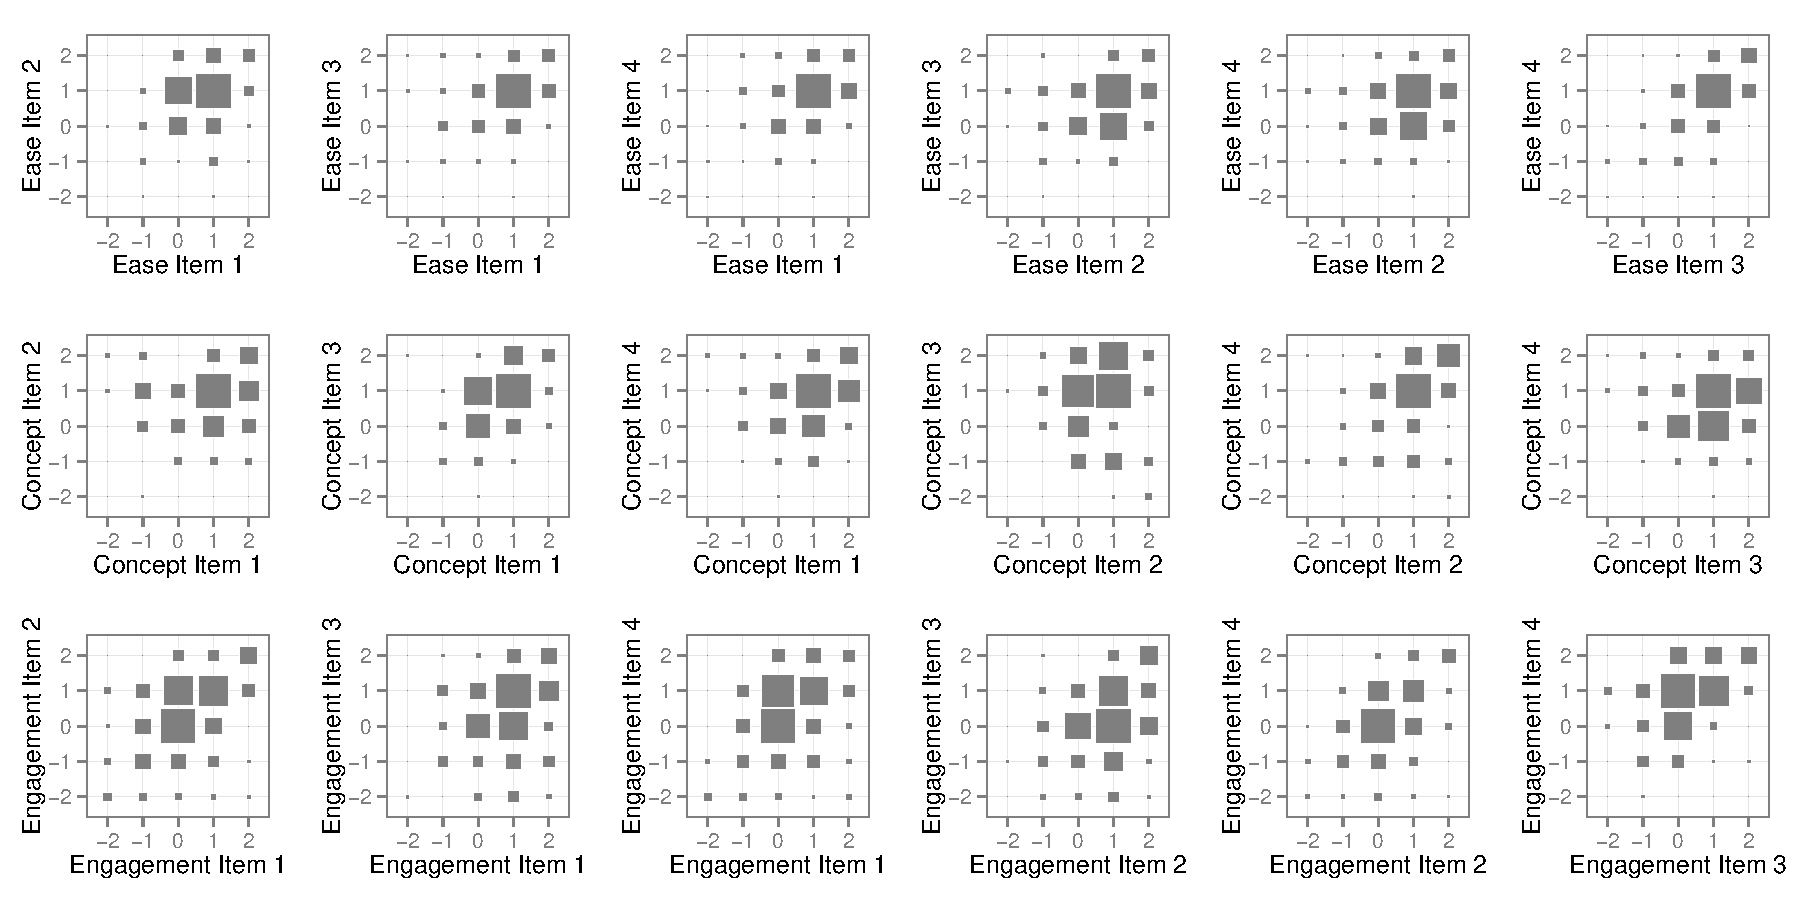
\includegraphics[width=.98\linewidth]{figure/fluctuationDiagrams-1} 

}

\caption[Fluctuation Diagrams of All Item Pairs within Topic Sets]{Fluctuation Diagrams of All Item Pairs within Topic Sets\label{fig:fluctuationDiagrams}}
\end{figure}


\end{knitrout}



Cronbach's $\alpha$ measures internal consistency between a set of responses by comparing the sum of individual variances to the variance of the sum of the responses. It is defined as follows

\begin{equation} \label{eq:alpha}
\alpha \cdot (K-1)/K =  1- \left . \sum_{i=1}^K \V{Y_i} \right /  \V{\sum_{j=1}^K Y_j},
\end{equation}

where $Y_i$ denotes the response on the $i^{\text{th}}$ survey item ($ i = 1,... , K$), and $K$ is the number of survey items considered for internal consistency. Generally, $K=4$ for the item sets of this survey.
Cronbach's $\alpha$ reaches a maximal value of 1, if there is perfect agreement between items (i.e. all responses to the same item set are identical). In the case that items sets are independent, the internal consistency is measured as $\alpha = 0 $. Cronbach's $\alpha$ is negative int the situation of consistent disagreement between responses and will approache negative infinity if there is perfect disagreement between items.  See appendix~\ref{appendCronbach} for details on the bounds for $\alpha$. 
 \citet[][p.~265]{Nunnally1978} propose that an $\alpha$ of 0.7 or above should be considered as an indication of ``modest reliability''.   \citet{GeorgeMallery2003} provide the commonly used extended scale, displayed in Table~\ref{GMAlphaScale}, for interpreting internal consistency based on Cronbach's $\alpha$. \\

\begin{table}[H]
\centering
\begin{tabular}{ll}
\hline 
Internal Consistency & Range \\
\hline
Excellent &  $[ 0.9 , 1.0 ]$ \\
Good & $[ 0.8 , 0.9 )$ \\
Acceptable & $[ 0.7 , 0.8 ) $\\
Questionable & $[ 0.6 , 0.7 )$ \\
Poor & $[ 0.5 , 0.6 )$ \\
Unacceptable & $( -\infty, 0.5 )$ \\
\hline
\end{tabular}
\caption{Extended Scale for Cronbach's $\alpha$ \citep{GeorgeMallery2003}.} 
\label{GMAlphaScale}
\end{table}

\hh{'are available' is a bit vague. Could you re-phrase this and say what distribution $\alpha$ follows under normality of the item sets? } \km{Is this better? the construction of the degrees of freedom for the F distribution are quite convoluted, but I have tried to boil down the primary origins}\\

\km{  Under the assumption of Gaussian data, the distribution of alpha is approximately $F_{\nu_1,\nu_2}$ distributed, where $\nu_1 = n-1$ and $\nu_2$ is based on a function of the eigenvalues from the quadratic linear combination of the roots of the variance matrix. \citep{KistnerMuller2004}.  Thus distributionally based confidence intervals are available for Cronbach's $\alpha$, but we are not entirely willing to assume Normally distributed responses to our survey and thus have elected to bootstrap the intervals instead.\\  }


Table~\ref{cronbachstuff} displays the point estimates and 95\% central bootstrap intervals for Cronbach's $\alpha$ for each item set from the student survey.  The intervals were created using quantiles of Cronbach's $\alpha$ values from each item set based on 10,000 bootstrap resamples. 
 The results indicate modest levels of internal consistency for Ease and Engagement item sets, and a lower level for the Concept item set. This is in agreement with the findings based on the fluctuation diagrams in Figure~\ref{fig:fluctuationDiagrams}. 



% latex table generated in R 3.0.2 by xtable 1.7-3 package
% Tue Nov 04 15:05:46 2014
\begin{table}[hbtp]
\centering
\begin{tabular}{lrc}
  \hline
Set & Estimate & 95\% Confidence Interval \\ 
  \hline
Ease & 0.70 & (0.613 , 0.759)\\ 
  Concept & 0.53 & (0.410 , 0.637) \\ 
  Engagement & 0.72 & (0.643 , 0.776) \\ 
   \hline
\end{tabular}
\caption{Cronbach's $\alpha$ Estimates for each item set with 95\% central confidence intervals based on 10000 bootstrap samples} 
\label{cronbachstuff}
\end{table}

\subsubsection{Assessment of Polarity Issues}  

We next turn our attention to the polarity of the survey items; specifically we consider that positive and reverse-scored negative items may elicit a different responses.  

The survey contained six unique item pairs based on topic and polarity combinations. Figure~\ref{fig:OverallSetBars} displays compares the distribution of responses from positive and negative item pairs within topics.  We see strong similarity between positive and reverse-scored negative items in response distributions with the Ease and Engagement item sets. The Concept item set however displays a noticeable difference in response distributions from each polarity.  In particular, we see that students are more neutral toward the positively worded questions. This polarity difference in student responses may explain the lower internal consistency measured by Cronbach's $\alpha$. This might be partly due to the problem that the negation of positive constructs may be linguistically counter-intuitive \citep{Friborg2006}. For instance, students may not interpret the statement ``It is not less clear'' as equivalent to the statement ``It is more clear''.  

\begin{knitrout}
\definecolor{shadecolor}{rgb}{0.969, 0.969, 0.969}\color{fgcolor}\begin{figure}[hbt]


{\centering 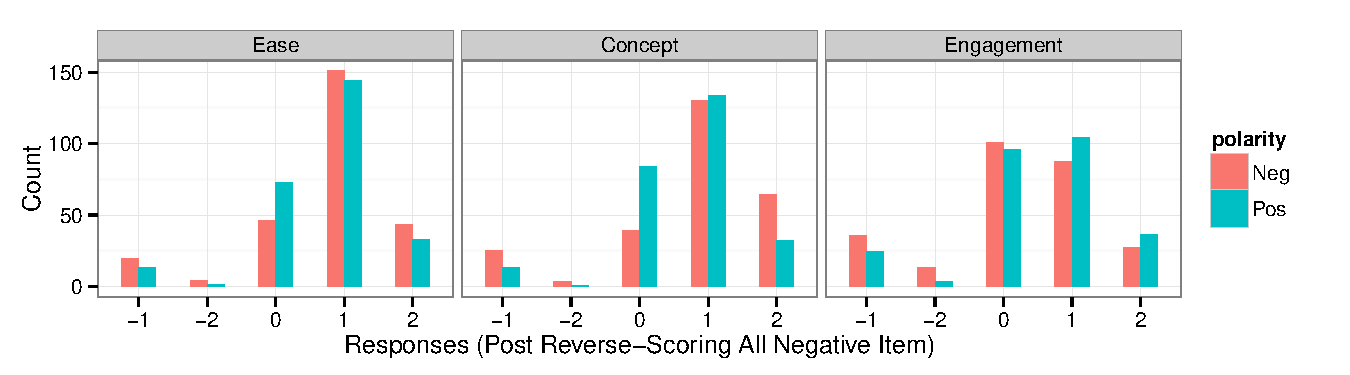
\includegraphics[width=.8\linewidth]{figure/OverallSetBars-1} 

}

\caption[Item set response distributions]{Item set response distributions\label{fig:OverallSetBars}}
\end{figure}


\end{knitrout}


To assess whether responses from positive and reverse-scored negative items can be reasonably grouped together within topic sets we turn to principal component analysis.  We decompose the item pairs averages for student responses from the six topic and polarity combinations. The component variances and factor loadings from this decomposition are found in Table~\ref{pc6table}. We argue that the data could be reasonably reduced to four principal components because each of these components explains over 10\% of the variance and together they explain 87.4\% of the total variation.  The uniformly aligned factor loadings for Component 1 reflect the general tendency toward student agreement to all items on the survey.  The factor loadings for Components 2 and 3 displayed in Figure~\ref{fig:PCA6plot} show similar projections for positive and negative item scores for Ease and Engagement pairs but a dramatic separation in the positive and negative item scores for the Concept set.  \\  



\begin{table}[H]
\centering
\begin{tabular}{lrrrrrrr}
\hline 
& Principal Component & 1 & 2 & 3 & 4 & 5 & 6 \\ 
\hline
Variances \hspace{.1in} & Prop. of Var & 0.457 & 0.181  & 0.135 & 0.101 & 0.071 & 0.055  \\
& Cumu. Prop. of Var & 0.457 & 0.638  & 0.773 & 0.874 & 0.945 & 1.000  \\
\hline
Loadings & Pos. Ease & -0.292 & 0.169 & -0.509 & -0.036 & -0.055 & 0.789\\
& Neg. Ease &  -0.444 & -0.390 & -0.464 & 0.429 & 0.372 & -0.335\\
& Pos. Concept &  -0.304 & 0.330 & -0.389 & -0.350 & -0.537 & -0.487\\
& Neg. Concept &  -0.408 & -0.641 & 0.250 & -0.585 & -0.067 & 0.116\\
& Pos. Engaged &  -0.367 & 0.523 & 0.207 & -0.321 & 0.663 & -0.083\\
& Neg. Engaged &  -0.569 & 0.164 & 0.519 & 0.496 & -0.355 & 0.087\\
\hline
\end{tabular}
\caption{Summary Statistics from Principal Component Analysis with Six Topic/Polarity Item Pairs} 
\label{pc6table}
\end{table}

\begin{knitrout}
\definecolor{shadecolor}{rgb}{0.969, 0.969, 0.969}\color{fgcolor}\begin{figure}[hbt]


{\centering 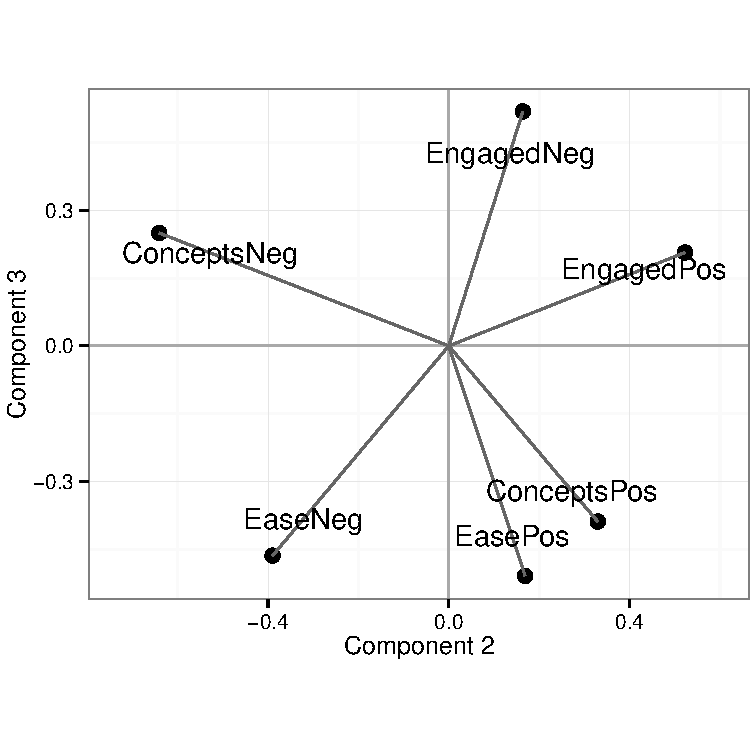
\includegraphics[width=.5\linewidth]{figure/PCA6plot-1} 

}

\caption[Item Pair Loadings on Components 2 and 3 from the Principal Component Analysis with Six Topic/Polarity Item Pairs]{Item Pair Loadings on Components 2 and 3 from the Principal Component Analysis with Six Topic/Polarity Item Pairs\label{fig:PCA6plot}}
\end{figure}


\end{knitrout}



This principal component analysis, with all topic and polarity combinations, suggests that we can reduce the dimensionality by combining the positive items with the reverse-scored negative items for Ease and Engagement topics.  This leaves only the Concept item set separated based on polarity for final analysis.  The decision to combine the responses for Ease and Engagement items also aligns with the higher internal consistency for these item sets as displayed in Cronbach's $\alpha$ values and fluctuation diagrams in Figure~\ref{fig:fluctuationDiagrams}. Thus, we will carry forward with the final analysis using four resulting item sets: Ease, Positive Concept, Negative Concept and Engagement.  

\subsubsection{Assessment of Orthogonality} 

The next major consideration is whether the item sets are truly measuring different latent topics and are not redundant. The ability of the survey to separately measure the topics of Ease, Concepts and Engagement can be assessed through the orthogonality of the responses from different item sets.  To check the orthogonality of the sets we conduct another principal component analysis; this time on the average responses for each student from the four item sets -- Ease, Positive Concept, Negative Concept and Engagement.  Items sets will be considered highly orthogonal if the principle component analysis cannot reduce the dimensionality from the four sets. \\  




\begin{table}[ht]
\centering
\begin{tabular}{lrrrrr}
\hline 
& Principal Component & 1 & 2 & 3 & 4 \\ 
\hline
Variances \hspace{.1in} & Prop. of Var & 0.515 & 0.249  & 0.134 & 0.102  \\
& Cumu. Prop. of Var & 0.515 & 0.764  & 0.898 & 1.000  \\
\hline
Loadings & Ease & -0.430 & 0.144 & -0.307 & 0.837\\
& Pos. Concept &  -0.408 & 0.562 & -0.520 & -0.497\\
& Neg. Concept &  -0.619 & -0.745 & -0.101 & -0.227\\
& Engagement &  -0.515 & 0.330 & 0.790 & -0.031\\
\hline
\end{tabular}
\caption{Principal Component Analysis with Final Four Item Sets} 
\label{pctable}
\end{table}

Table~\ref{pctable} displays the proportion of variance explained by each of the four principal components and also the loadings for each item set mean that compose each component. The first principal component has similar loadings from all item sets, which we can interpret as the general tendency toward positively scored responses on all items. The second, third and fourth principal components create separation for mean responses of the Negative Concept item set, the Engagement item set and the Ease item sets, respectively. The variances in Table \ref{pctable} reveal that over 10\% of the variation is explained by the fourth component, thus it is necessary to retain all four principal components. This inability to reduce dimensionality implies that average student responses from the four item sets are largely orthogonal. Based on the separation in the loadings and the orthogonality of the principal components, we conclude that the average response scores from the four item set have interpretability as measurements of unique latent topics. \\  


%-------------------------------------------------------------------------
\subsubsection{Survey Assessment Results} 

\km{  In the analysis of student responses, we found that the internal consistency, assessed with Cronbach's $\alpha$ and fluctuation diagrams, is acceptable for interpreting the combined item responses that measure of Ease of Use and Engagement with the census data. We did not have the same certainty with the measures of Concept and therefore split the Concept items into two sets: the Positive and Negative Concept item sets.  This split is supported by the initial principal component analysis of the six topic and polarity item pair scores.  The follow-up principal component analysis on the combined responses for each of the four resulting item sets indicated that the factors were all fairly orthogonal. This ensures us that the survey was effective at eliciting unique characteristics of the user experience. \\  }

\km{ The barcharts found in Figure \ref{fig:OverallSetBars} show that the distribution for each item set is heavily skewed to the left, with the majority of students having the neutral to positive responses. The small bump at the far left of each distribution indicates that there was a small minority of students that expressed negative views. The response distributions indicate that on average students found the application easy to use, found that the tool connected them to sampling concepts and felt moderately engaged with the census data that was accessed with the application.  \\  }


%-------------------------------------------------------------------------
%\km{ \subsubsection{Conclusions} }


\newpage

%-----------------------------------------------------------------------------------
\section{Shiny Database Aggregator}
Brief intro the functionality goals for the tool


%%%-----------------------------------------------------------------------------------
\subsection{Layout and Functionality}
To be determined

%%%-----------------------------------------------------------------------------------
\subsection{Applications}
To be determined



%-----------------------------------------------------------------------------------
\section{Conclusions and Future Work}


%------------------------------------------------------------------
% References
\bibliographystyle{asa}
\bibliography{references}

\newpage
%-------------------------------------------------------
\appendix
%-------------------------------------------------------
\section{Appendix: Lab Assignment}
\label{labappend}

For this activity you will be using a tool called the Shiny Database Sampler to take a random sample of United States residents from US census data. The census data is the Public Use Microdata Sample (PUMS) which is a 3 million person subset of the entire Census data.  For this activity we treat our samples as though they are selected from the full census records.  \\ 
	
We are going to explore how these random sampling plans relate to the goals of a sample survey. The tool will allow you to define either a simple random sampling plan or a stratified random sampling plan. In the following two scenarios we will explore the advantages and disadvantages of these two sampling plans. Access the tool at \url{http://shiny.stat.iastate.edu/karstenm/ShinyDatabaseSampler}. \\	 

\underline{Scenario 1:} Suppose that our goal is to estimate the mean age of all US residents. Similar to polling organizations we have a budget that allows us to survey around 1000 people. To collect our sample we decide to take a simple random sample of 1040 US residents. \\

\begin{enumerate}[(a)]
\item Is this study and example of an experiment or an observational study?  Explain your answer.
\item	Your colleague Bob claims that we are wasting our budget to get only 1040 people using random sampling. He says that we could get 20000 responses to the survey if we invested that money into a mailing campaign in Minneapolis. Explain why the random selection is important.
\item	Another colleague, Jill, asks why we do not stratify by state when we take the sample so that we get 20 people from each of the 50 states along with Puerto Rico and the District of Columbia. Explain why this idea would not create a representative sample to pursue our goal.
\end{enumerate}

Now that we have decided on our sampling plan, let's go collect our data.  The Shiny Database Sampler needs to be told 4 pieces of information in order to collect census records the way you want. (1) Choose the database called ``Census'', (2) select the ``simple random sample'' option, (3) enter a random seed, any number between 1 and 10000, you can do this by rolling a 10-sided die 4 times and (4) lastly tell it that we want ``1040'' random draws. Once you have drawn your samples the page will display basic summary statistics for the variables in the census.\\

\begin{enumerate}[(a)]
\setcounter{enumi}{3}
\item Report the 5-number summary and sample mean age.
\item	Use the 5-number summary to construct a box plot of age.
\item	Go to the ``Basic Plots of Your Sample'' tab.  Choose age as your Response Variable to Plot.  What type of variable is this?  By clicking on Make My Plot? a histogram of the sample of ages will be displayed.  Describe the shape of the data distribution of age.
\item	Is the relationship between the sample mean and sample median consistent with your description of shape?  Explain briefly.
\item	If our goal was to not only estimate the mean age of all the U.S. residents but also come up with estimates of the median age of all residents in each of the 50 states, plus the District of Columbia and Puerto Rico what is a drawback of using the simple random sample of 1040?  Hint: Set the Data Table to display 100 records per page and go to the page that has ``states'' 10 and 11 (Delaware and the District of Columbia).
\end{enumerate}

\underline{Scenario 2:} Suppose now that our goal has changed.  Now we wish to investigate the association between age and state of residency. We want to compare the median ages for different states. We still have a budget that allows us to survey around 1040 people. To collect our sample we decide to take a stratified random sample of 20 residents from each state in the United States plus the District of Columbia and Puerto Rico. 

\begin{enumerate}[(a)]
\setcounter{enumi}{8}
\item  Explain in general why collecting a stratified random sample is a better plan than a simple random sample for answering this question.  
\end{enumerate}

Now that we have decided on our new sampling plan, let's go collect our data.  The Shiny Database Sampler will need to be told 5 pieces of information in order to collect census records the way you want this time. (1) Choose the database called ``Census'', (2) select the ``stratified random sample'' option, (3) enter a random seed, any number between 1 and 10000, you can do this by rolling a 10-sided die 4 times, (4) select ``state'' as strata variable and (5) lastly tell it that we want ``20'' random draws from each state, plus the District of Columbia and Puerto Rico.  \\

It will take a minute or two to collect these data. It is sifting through millions of records and randomly selecting them from within state groups after all! Once you have drawn your samples you can take a peek at your data set in the main panel of the webpage. You will be able to answer the following questions using the summaries provided on the webpage.  \\

You will notice that the summaries are all broken down by state, but the states are not given names, they are given a code number.  This is done on the census to save computer storage space (saving a ``19'' is much smaller than ``Iowa'').  A list of all the state codes is available at \url{https://www.census.gov/geo/reference/ansi\_statetables.html} (Click on FIPS Codes for the States and the District of Columbia).\\ 



\begin{enumerate}[(a)]
\setcounter{enumi}{9}
\item Report the mean and 5-number summary for the age of the sample from the state of Iowa (\texttt{state = 19}).
\item	Report the mean and 5-number summary for the age of the sample from the state of Alaska (\texttt{state = 2}).
\item	Compare the distribution of ages in Alaska and Iowa using the values from parts j and k.
\item	Making comparisons as we have done above would become tedious if we wanted to compare ages between all pairs of states in the country.  What would be a good way to visually display this information so aid in making these comparisons? Explain your answer.
\end{enumerate}


%------------------------------------------------------------------
\section{Appendix: Database Descriptions}
\label{appendDB}

\textbf{To be detailed when databases updated and origins better known.}

%------------------------------------------------------------------
\section{Appendix: Cronbach's $\alpha$ Properties}
\label{appendCronbach}

\km{

Recall the form of Cronbach's $\alpha$ from equation~(\ref{eq:alpha}):\\

\begin{center}
$\alpha = \left(K/(K-1)\right) \left( 1- \sum_{i=1}^K \V{Y_i} \right.\left/  \V{\sum_{j=1}^K Y_j}  \right)$,
\end{center}


\textit{Claim 1:} Perfect agreement in items leads to $\alpha = 1$ \\

\textit{Proof:} Let $ Y = Y_1 = Y_2 = ... = Y_k$, thus having perfect agreement.\\

$\Rightarrow$  $\text{Cov}(Y_i, Y_j) = \V{Y} = \sigma^2_y $ \hspace{.1in} $\forall i\ne j$ \\

$\Rightarrow$  $\V{\sum_{j=1}^K Y_j }$ = $\sum_{i=1}^K \V{Y_i} + \sum_{i\ne j}\text{Cov}(Y_i, Y_j)$ =  $K\sigma^2_y + K(K-1)\sigma^2_y$ \\

$\Rightarrow$  $\alpha = \left(K/(K-1)\right) \left( 1- \sum_{i=1}^K \V{Y_i} \right.\left/  \V{\sum_{j=1}^K Y_j}  \right)$ = \\
\indent \hspace{.2in} $\left(K/(K-1)\right) \left( 1- K\sigma^2_y \right.\left/ K\sigma^2_y + K(K-1)\sigma^2_y \right)$ =\\
\indent \hspace{.2in} $\left(K/(K-1)\right)  (1- 1/K)$ = $\left(K/(K-1)\right) ((K-1)/K)$ = $1$ \\

\vspace{.25in} %------------------------------

\textit{Claim 2:} For independent items $\alpha = 0$ \\

\textit{Proof:} Let $Y_1 = Y_2 = ... = Y_k$ be independent 

$\Rightarrow$ $\sum_{i=1}^K \V{Y_i} = \V{\sum_{j=1}^K Y_j} $ \\

$\Rightarrow$  $\alpha = \left(K/(K-1)\right) \left( 1- \sum_{i=1}^K \V{Y_i} \right.\left/  \V{\sum_{j=1}^K Y_j}  \right)$ = \\
\indent \hspace{.2in} $\alpha = \left(K/(K-1)\right) \left( 1- \V{\sum_{j=1}^K Y_j} \right.\left/  \V{\sum_{j=1}^K Y_j}  \right)$ = \\
\indent \hspace{.2in} $\alpha = \left(K/(K-1)\right) \left( 1- 1 \right)$ = 0 \\

\vspace{.25in} %------------------------------

\textit{Claim 3:} Perfect disagreement in items leads to $\alpha = -\infty$ \\

\textit{Proof:} Let $K=2$ and $Y_1 = -Y_2$, thus having perfect disagreement.\\

$\Rightarrow$  $\V{Y_1 + Y_2}$ = $\V{Y_1 - Y_1}$ = $\V{0}$ = $0$

$\Rightarrow$  $\alpha = \left(K/(K-1)\right) \left( 1- \sum_{i=1}^K \V{Y_i} \right.\left/  \V{\sum_{j=1}^K Y_j}  \right)$ = $(2/1)(1-2\sigma^2_y/0)$ = $-\infty$ \\

} %end km

\end{document}
